\subsection*{COMPARACIÓN ENTRE TODAS LAS MÉTRICAS INDIVIDUALES}
\label{sec:metricas-individuales}

Comparación para métrica de calidad de señal:
\begin{figure}[H]
  \centering
  \centerline{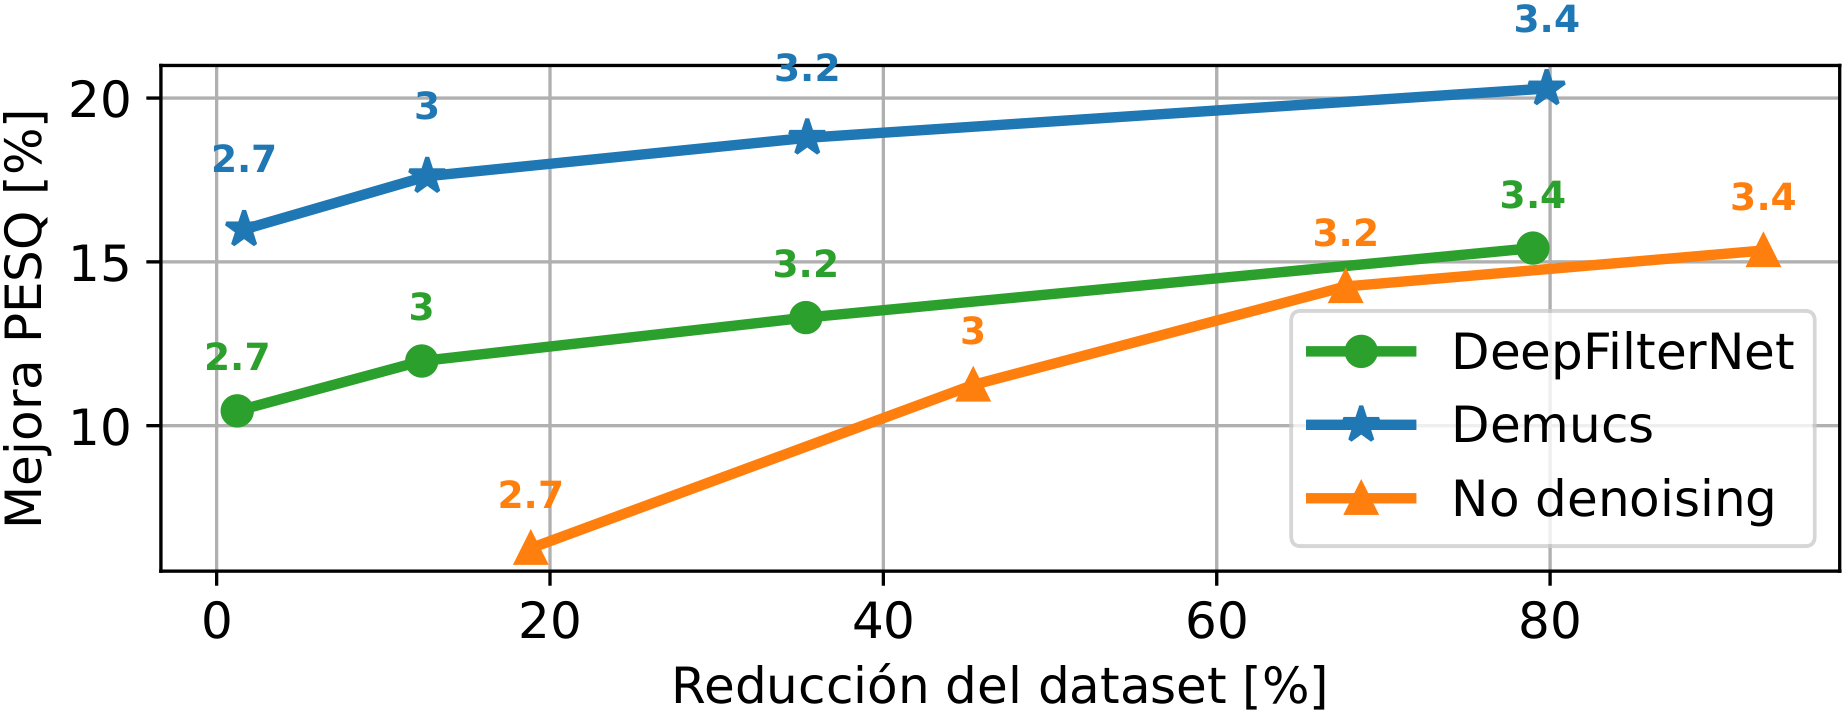
\includegraphics[width=11cm]{Figuras/Anexo-I/PESQ vs hours (dnsmos)_page1.png}}
  \caption{Comparación entre PESQ y horas del dataset para diferentes variantes con DNSMOS.}
\end{figure}

\begin{figure}[H]
  \centering
  \centerline{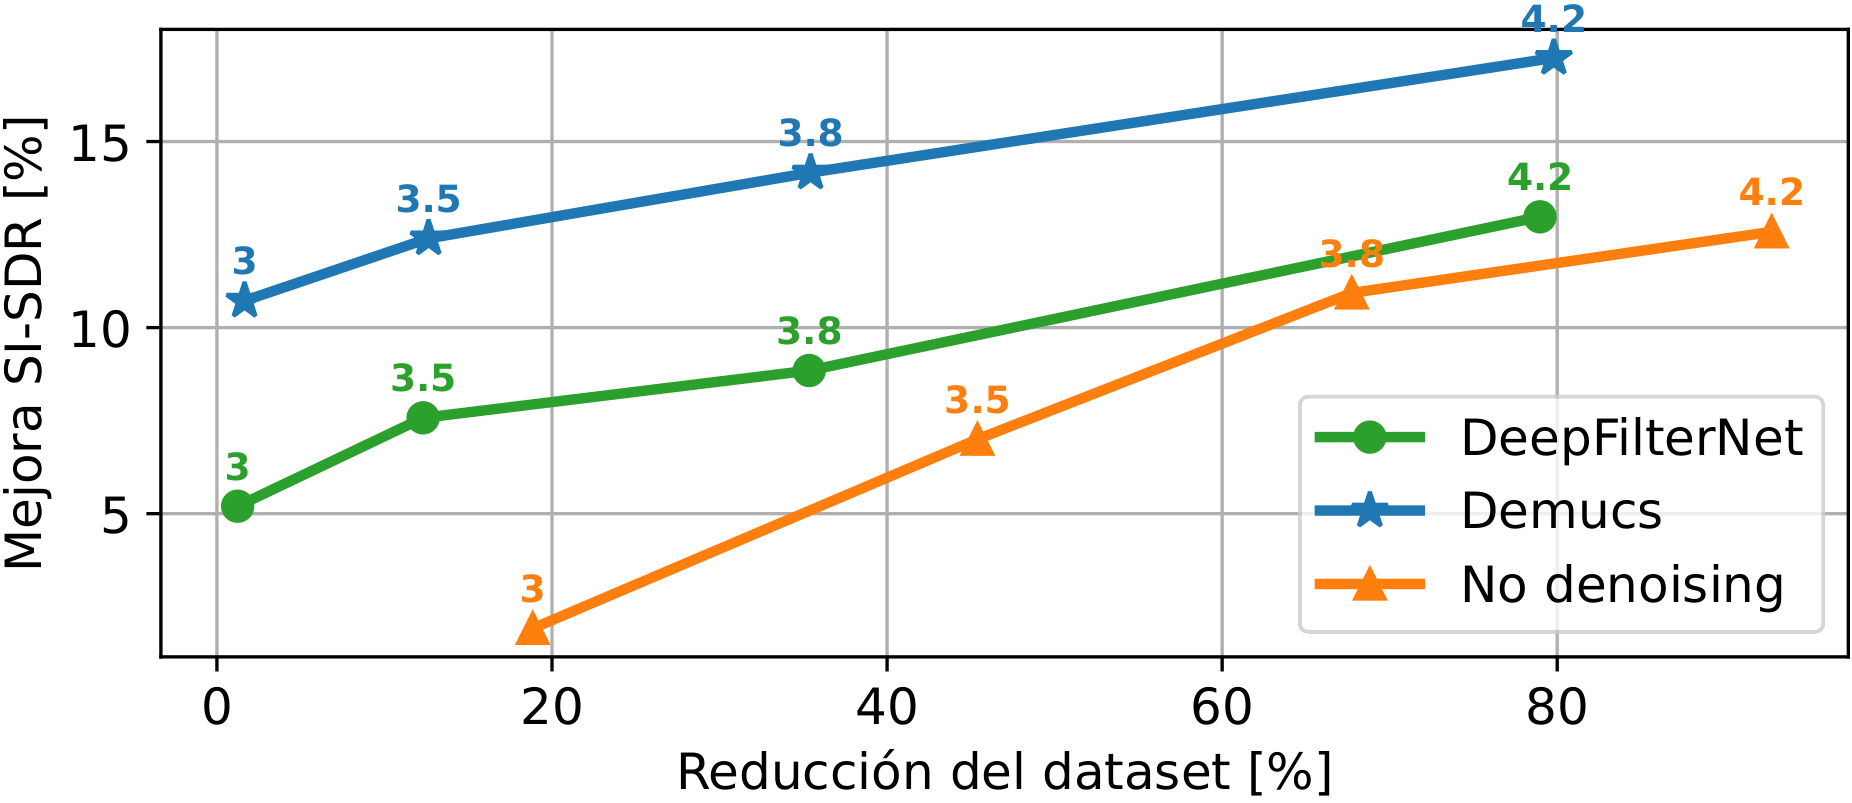
\includegraphics[width=11cm]{Figuras/Anexo-I/SI-SDR vs horas (dnsmos)_page1.png}}
  \caption{Comparación entre SI-SDR y horas del dataset para diferentes variantes con DNSMOS.}
\end{figure}

\begin{figure}[H]
  \centering
  \centerline{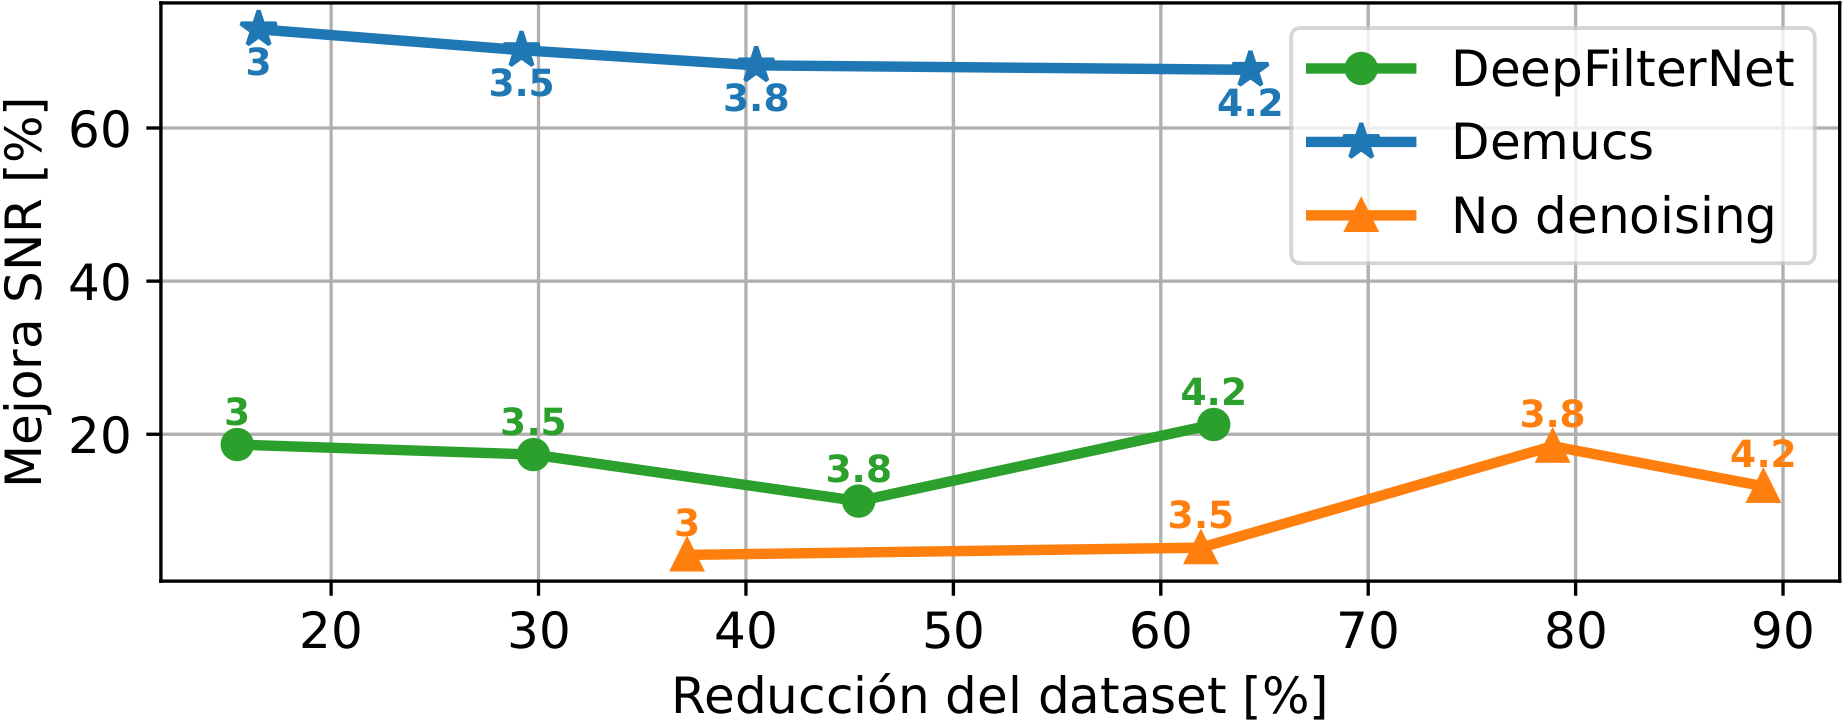
\includegraphics[width=11cm]{Figuras/Anexo-I/SNR vs horas (nisqa)_page1.png}}
  \caption{Comparación entre SNR y horas del dataset para diferentes variantes con NISQA.}
\end{figure}

Comparación para métrica de condiciones acústicas:

\begin{figure}[H]
  \centering
  \centerline{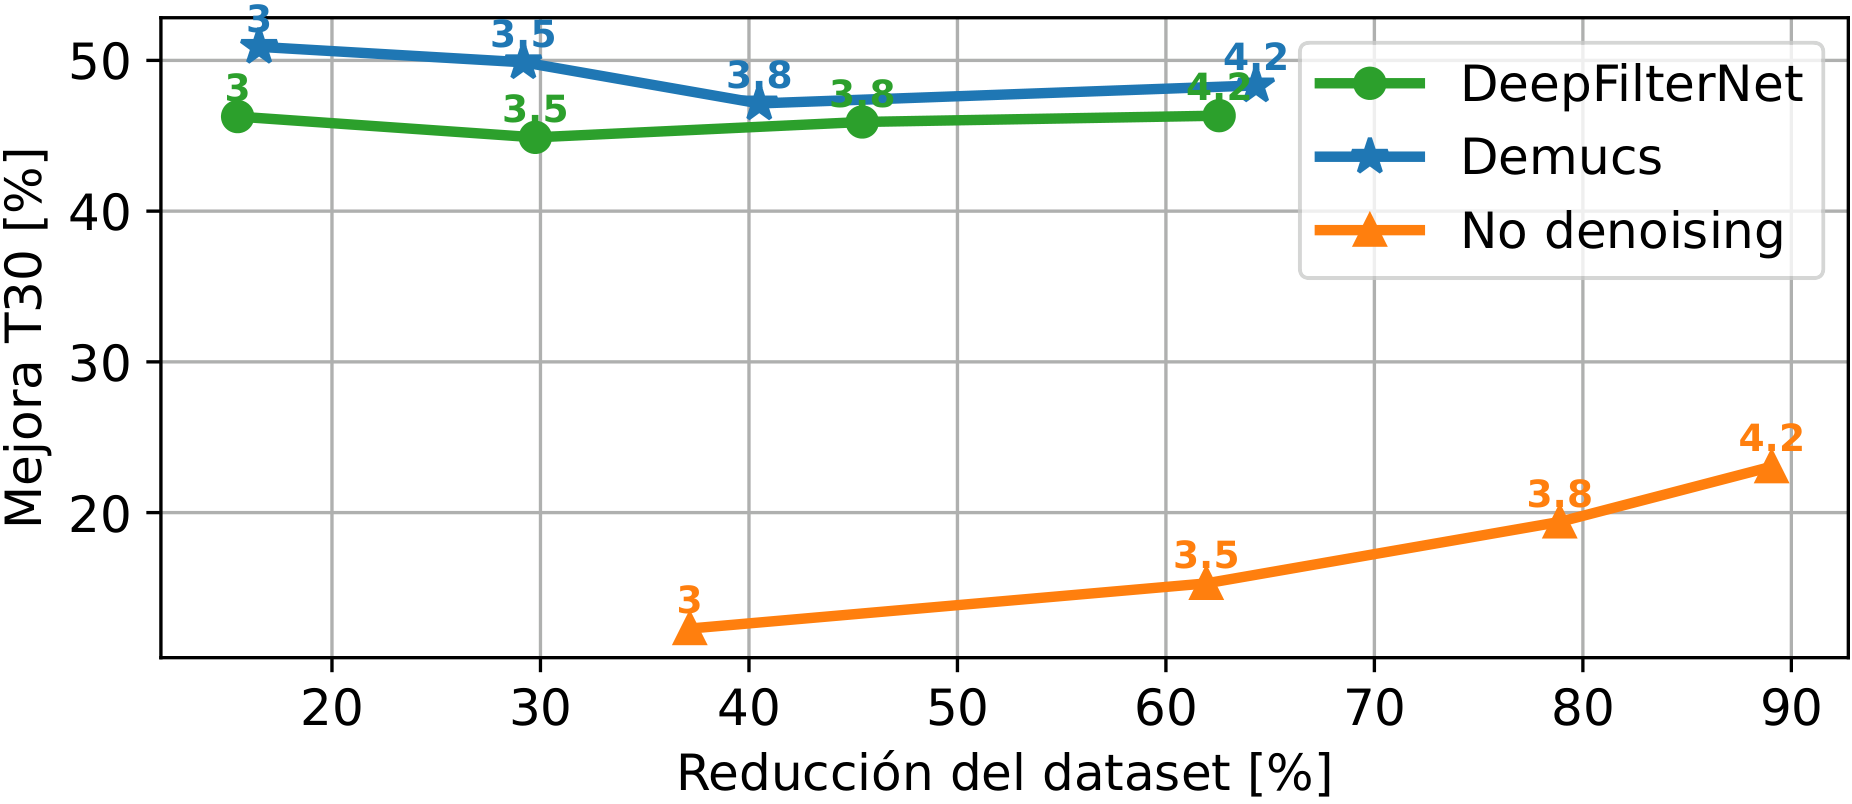
\includegraphics[width=11cm]{Figuras/Anexo-I/T30 vs horas (nisqa)_page1.png}}
  \caption{Comparación entre T30 y horas del dataset para diferentes variantes con NISQA.}
\end{figure}

\begin{figure}[H]
  \centering
  \centerline{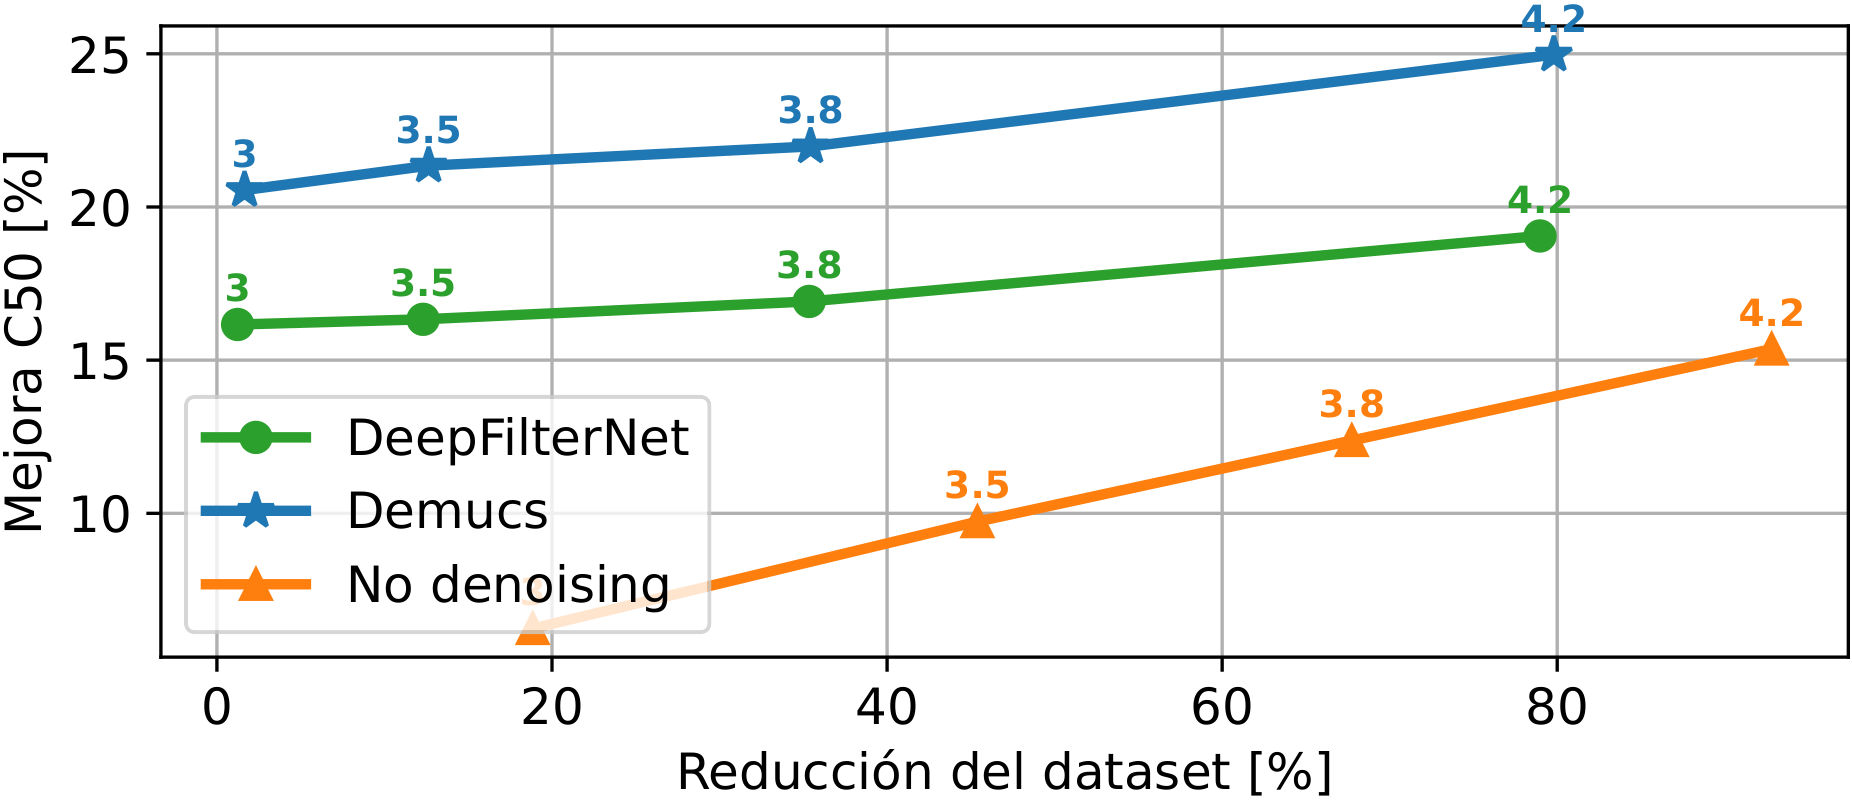
\includegraphics[width=11cm]{Figuras/Anexo-I/C50 vs horas (dnsmos)_page1.png}}
  \caption{Comparación entre C50 y horas del dataset para diferentes variantes con DNSMOS.}
\end{figure}

Comparación métrica de diferencias del hablante vs calidad de señal:

\begin{figure}[H]
  \centering
  \centerline{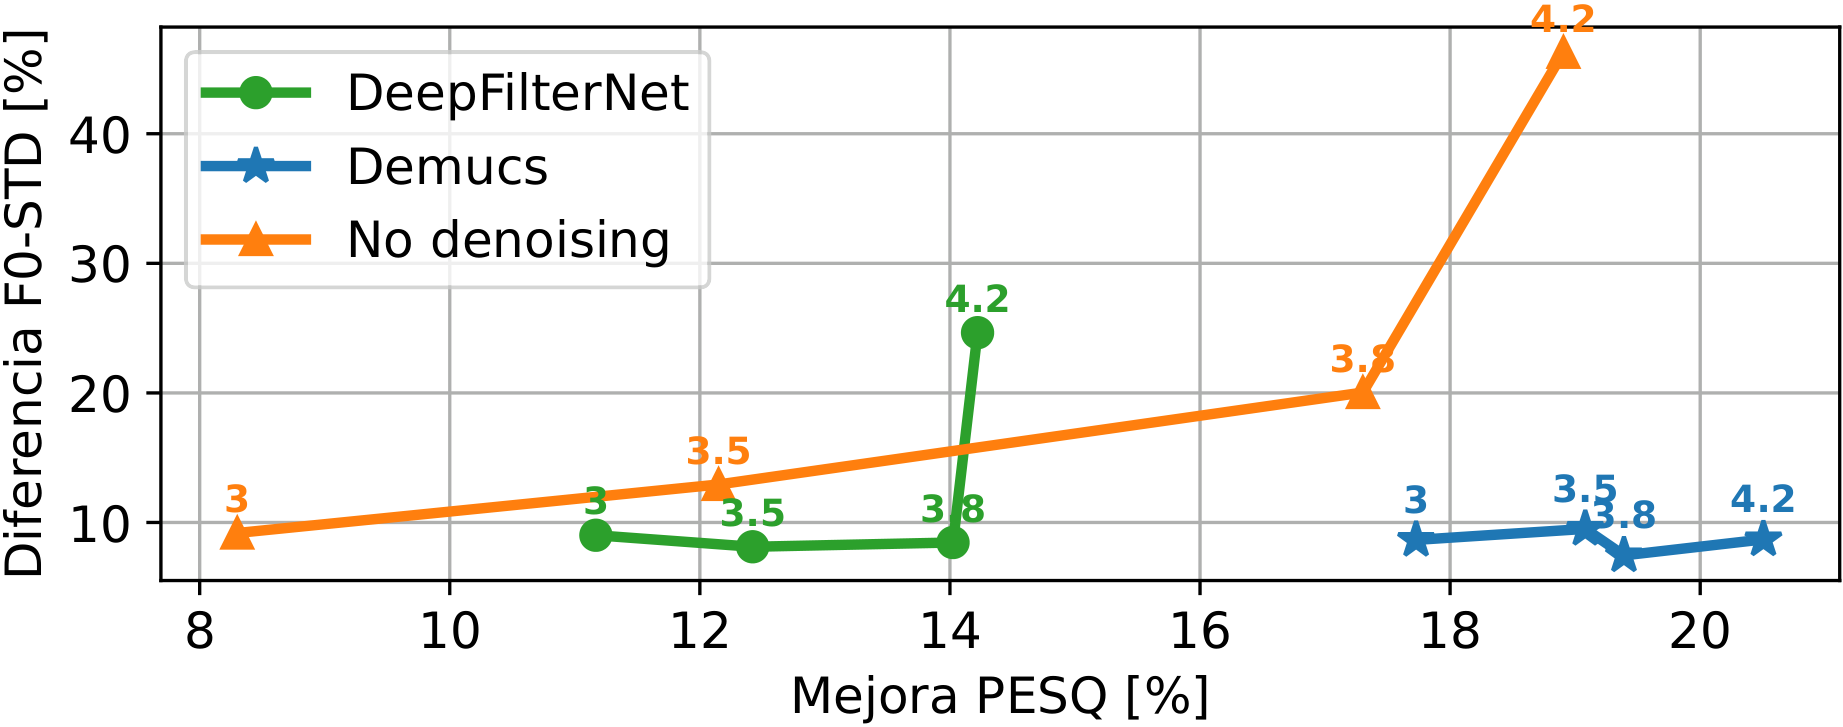
\includegraphics[width=11cm]{Figuras/Anexo-I/F0-STD vs PESQ (nisqa)_page1.png}}
  \caption{Comparación entre F0-std y PESQ del dataset para diferentes variantes con DNSMOS.}
\end{figure}

\subsection*{COMPARACIÓN ENTRE TODAS LAS MÉTRICAS COMPUESTAS}
\label{sec:metricas-compuestas}

\begin{figure}[H]
  \centering
  \centerline{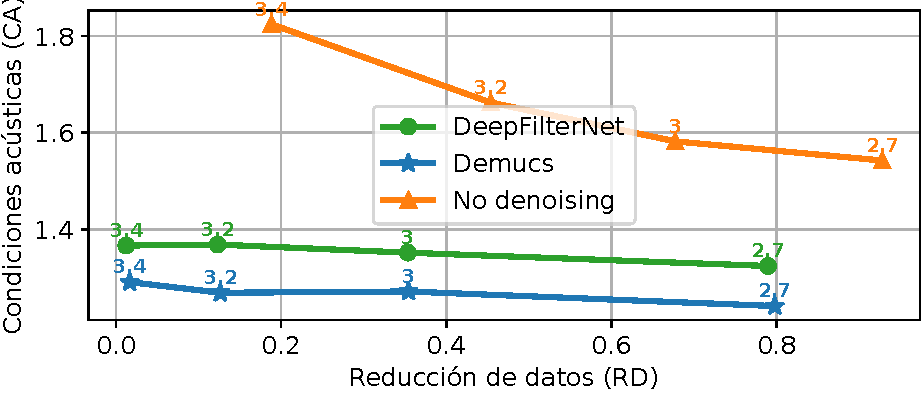
\includegraphics[width=11cm]{Figuras/Anexo-I/RD vs CA (dnsmos).pdf}}
  \caption{Comparación entre RD y CA del dataset para diferentes variantes con DNSMOS.}
\end{figure}

\begin{figure}[H]
  \centering
  \centerline{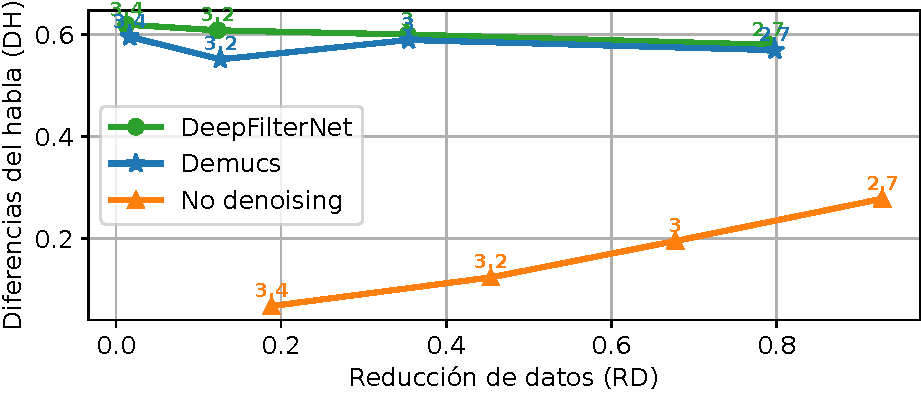
\includegraphics[width=11cm]{Figuras/Anexo-I/RD vs DH (dnsmos).pdf}}
  \caption{Comparación entre RD y DH del dataset para diferentes variantes con DNSMOS.}
\end{figure}

\subsection*{METRICAS COMPARACIÓN ENTRE DATASET ITW VS PROFESIONAL}
\label{sec:comparación-itw-vs-profesional}

\begin{figure}[H]
  \centering
  \centerline{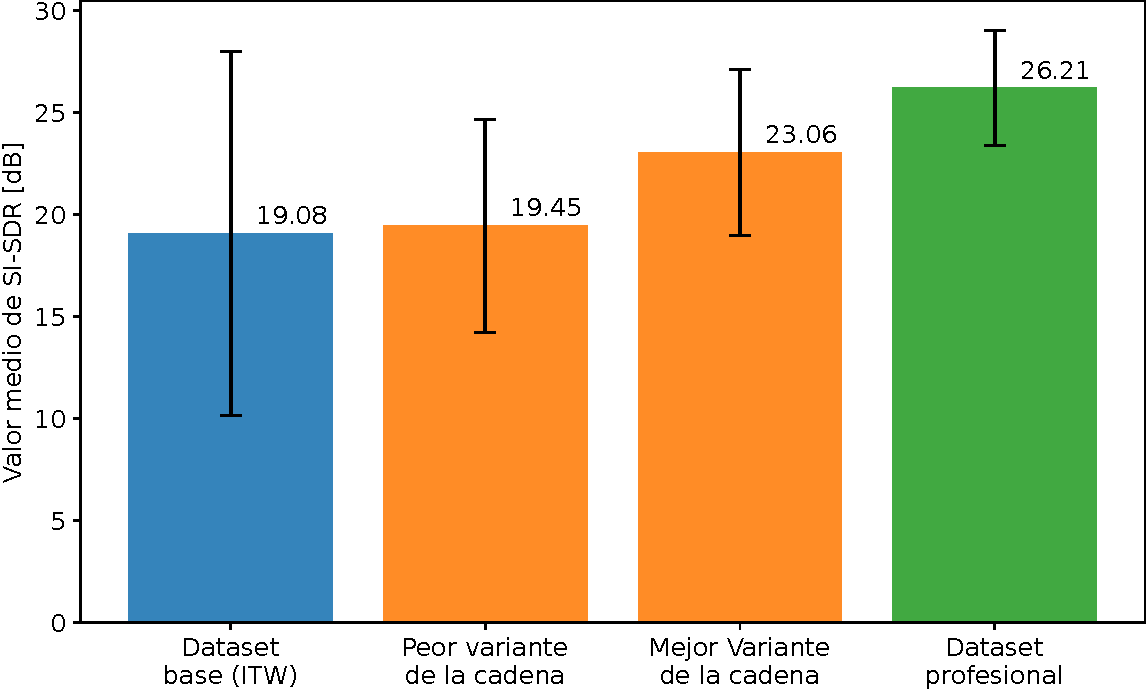
\includegraphics[width=11cm]{Figuras/Pro_vs_Pipe/Comparación tipos datasets SI-SDR.pdf}}
  \caption{Comparación entre SI-SDR de los datasets ITW y Profesional.}
\end{figure}

\begin{figure}[H]
  \centering
  \centerline{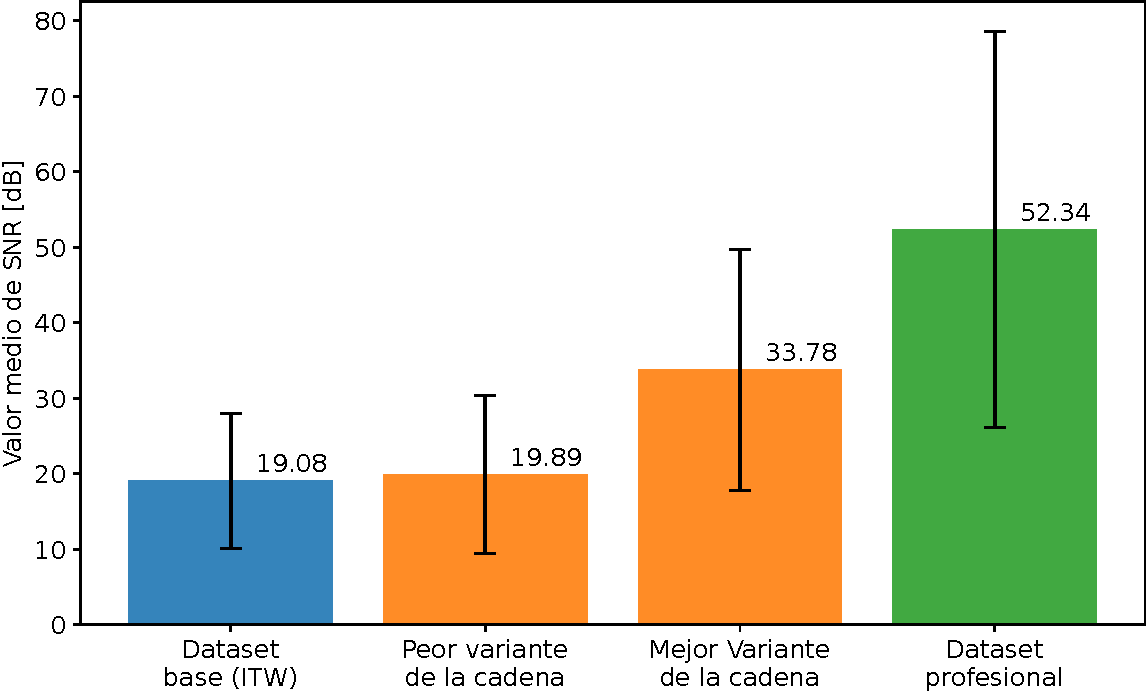
\includegraphics[width=11cm]{Figuras/Pro_vs_Pipe/Comparación tipos datasets SNR.pdf}}
  \caption{Comparación entre SNR de los datasets ITW y Profesional.}
\end{figure}

\begin{figure}[H]
  \centering
  \centerline{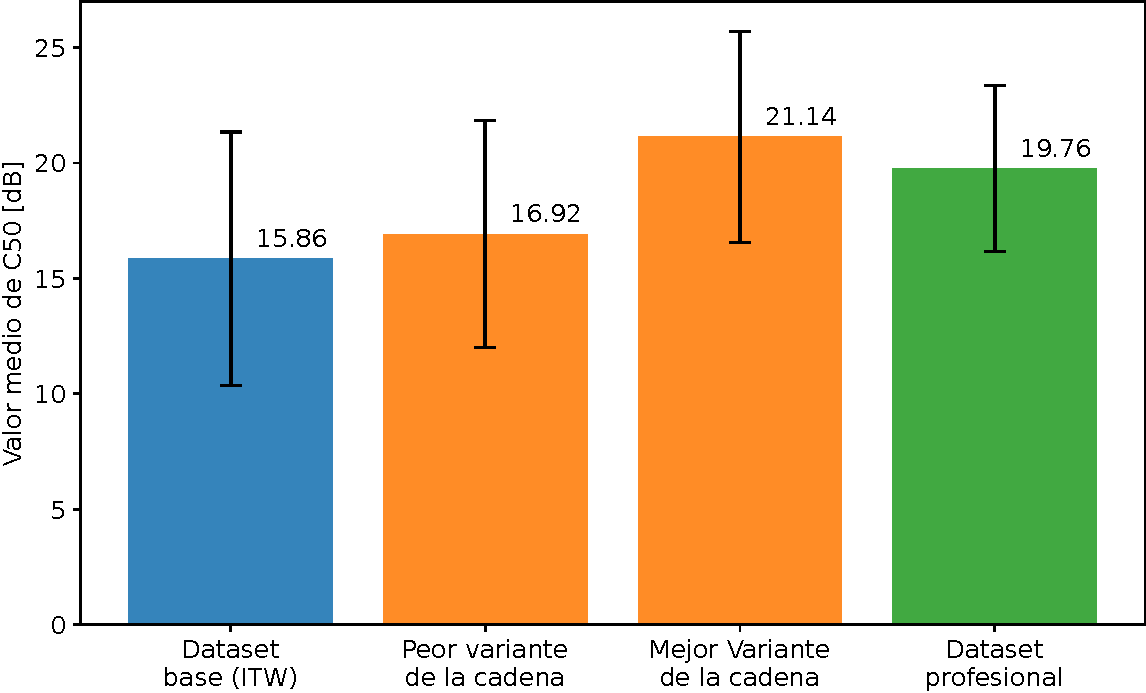
\includegraphics[width=11cm]{Figuras/Pro_vs_Pipe/Comparación tipos datasets C50.pdf}}
  \caption{Comparación entre C50 de los datasets ITW y Profesional.}
\end{figure}